\documentclass[tikz, border=10pt]{standalone}
\usepackage{amsmath}
\usetikzlibrary{positioning, fit, calc, arrows.meta, backgrounds}

\begin{document}

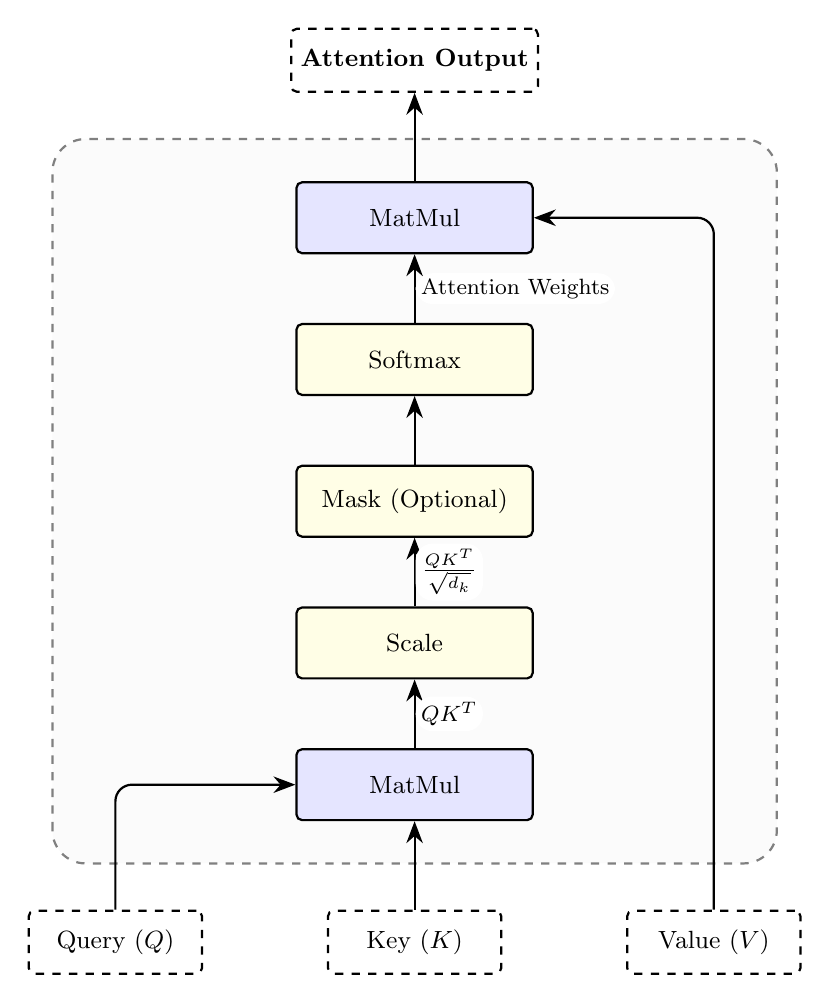
\begin{tikzpicture}[
    block/.style={draw, thick, rounded corners=2pt, minimum width=3cm, minimum height=0.9cm, text centered, font=\small},
    matmul/.style={block, fill=blue!10},
    norm/.style={block, fill=yellow!10},
    input/.style={draw, dashed, thick, rounded corners=2pt, minimum width=2.2cm, minimum height=0.8cm, text centered, font=\small},
    arrow/.style={-{Stealth[scale=1.2]}, thick, rounded corners=6pt},
    label/.style={font=\footnotesize, fill=white, inner sep=2pt}
]

% ----------------- 2. 放置节点 -----------------
% 底部输入节点 (绝对居中对称放置)
\node[input] (K) at (0, 0) {Key ($K$)};
\node[input] (Q) at (-3.8, 0) {Query ($Q$)};
\node[input] (V) at (3.8, 0) {Value ($V$)};

% 核心处理层 (拉大了垂直间距，完美解决公式遮挡问题)
\node[matmul] (matmul1) at (0, 2)   {MatMul};
\node[norm]         (scale)   at (0, 3.8) {Scale};           % 间距加大至2.2
\node[norm]         (mask)    at (0, 5.6) {Mask (Optional)}; % 间距加大至2.2，给分式留足空间
\node[norm]         (softmax) at (0, 7.4) {Softmax};         % 间距1.8
\node[matmul]    (matmul2) at (0, 9.2)  {MatMul};          % 间距1.8

% 顶部输出节点
\node[input, font=\small\bfseries] (output) at (0, 11.2) {Attention Output};

% ----------------- 3. 绘制连线与箭头 -----------------
% Q, K, V 输入连线 (|- 实现先直走再横走的直角平滑弯折)
\draw[arrow] (K) -- (matmul1);
\draw[arrow] (Q) |- (matmul1.west); 
\draw[arrow] (V) |- (matmul2.east); 

% 垂直主干连线，带有对应理论公式标签
\draw[arrow] (matmul1) -- node[label, right] {$Q K^T$} (scale);
% 带有大分式的公式现在有充足的纯白背景空间，不再触碰方框
\draw[arrow] (scale)   -- node[label, right] {$\frac{Q K^T}{\sqrt{d_k}}$} (mask);
\draw[arrow] (mask)    -- (softmax);
\draw[arrow] (softmax) -- node[label, right] {Attention Weights} (matmul2);
\draw[arrow] (matmul2) -- (output);

% ----------------- 4. 绘制居中的虚线背景框 -----------------
% 使用背景层绘制，确保绝对居中且不遮挡线条
\begin{scope}[on background layer]
    % 矩形从 x=-4.6 到 x=4.6 (严格对称)，y从 1 到 11 (包裹核心计算步骤)
    \draw[dashed, draw=gray, thick, rounded corners=12pt, fill=gray!3] (-4.6, 1) rectangle (4.6, 10.2);
\end{scope}

\end{tikzpicture}

\end{document}